\documentclass{article}
\usepackage[utf8]{inputenc}
\usepackage[letterpaper]{geometry}
\usepackage{amsmath}
\usepackage{bm}
\usepackage{algorithm}
\usepackage{algorithmic}
\usepackage{graphicx}
\usepackage{subcaption}
\usepackage{cleveref}

\linespread{1.2}

\title{Numerical Solution of Steady-State Heat Equation}
\author{Jiaqi Li}
\date{November 2018}

\begin{document}

\maketitle

% section on governing equations
\section{Governing Equations}

In this document, we attempt to solve the steady-state heat equation in one- and two- dimensions.
In 1D, we have
\begin{equation} \label{eq:heat_eq1d}
    -kT''(x) = q(x),\quad x \in \Omega
\end{equation}
In 2D, we have
\begin{equation} \label{eq:heat_eq2d}
    -k \nabla^2 T(x,y) = q(x,y),\quad (x,y) \in \Omega
\end{equation}
where $k$ is the thermal conductivity, $T$ is temperature, and $q$ is a given heat source term. To simplify the problem, we make the following 
assumptions:
\begin{itemize}
    \item $k$ is constant throughout the domain.
    \item $\Omega = (0,l)$ in 1D and $\Omega = (0, l) \times (0, l)$ in 2D.
    \item Dirichlet boundary condition:
        \begin{equation} \label{eq:bc}
            T|_{\partial \Omega} = g
        \end{equation}
        where $\partial \Omega$ denotes the boundary of domain $\Omega$, and $g$ is a given function defined on $\partial \Omega$.
\end{itemize}
From PDE theory we know that the combination of equation (\ref{eq:heat_eq1d})/(\ref{eq:heat_eq2d}) and (\ref{eq:bc}) forms a well-posed problem provided that $q$ and $g$ are smooth.


% section on discretization schemes
\section{Discretization Schemes}
Central difference is used to discretize the second-order derivative in the heat equation. 

\begin{figure}
    \centering
    \begin{subfigure}[t]{.5\textwidth}
        \centering
        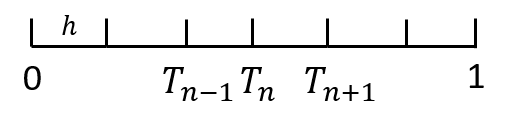
\includegraphics[width=0.9\linewidth]{1d_mesh.png}
        \caption{1D mesh}
    \label{fig:mesh1d}
    \end{subfigure}%
    \begin{subfigure}[t]{.5\textwidth}
        \centering
        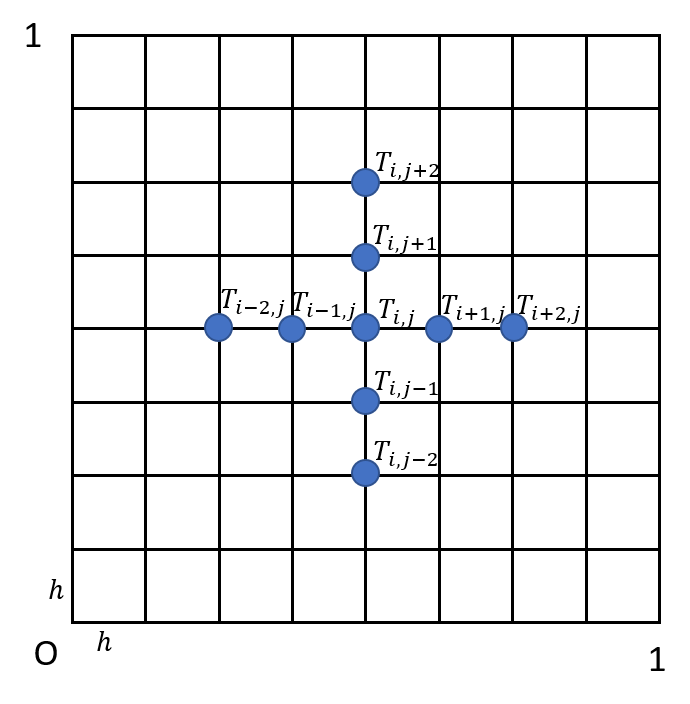
\includegraphics[width=0.9\linewidth]{2d_mesh.png}
        \caption{2D mesh}
    \label{fig:mesh2d}
    \end{subfigure}
    \caption{Representative figures of 1D and 2D mesh}
\label{fig:mesh}
\end{figure}

% 1D case
\subsection{1D case}
In 1D case, we partition the domain into uniform intervals, as sketched in Figure \ref{fig:mesh}(\subref{fig:mesh1d}).
Assume $0 = x_0 < x_1 < ... < x_m = l$, and $x_n - x_{n-1} = h,\  n = 1, 2, ..., m$.
The second-order approximation to the second-order derivative is
    $$T''(x_n) = \frac{1}{h^2}\left(T_{n-1} - 2 T_n + T_{n+1}\right) + O(h^2)$$
where $T_n = T(x_n)$.
Then the discrete approximation to equation (\ref{eq:heat_eq1d}) is
    $$\frac{1}{h^2}\left(T_{n-1} - 2 T_n + T_{n+1}\right) + O(h^2) = -\frac{q_n}{k}$$
where $q_n = q(x_n)$. In order to get an approximate solution, we neglect the second-order term, and obtain
\begin{equation} \label{eq:heat_eq1d_order2}
    T_{n-1} - 2 T_n + T_{n+1} = -\frac{q_n h^2}{k}, \quad n = 1, 2, ..., m-1
\end{equation}
The boundary condition (\ref{eq:bc}) implies
\begin{equation} \label{eq:bc_order2}
    T_0 = g(0), \quad T_m = g(1)
\end{equation}
Equations (\ref{eq:heat_eq1d_order2}) and (\ref{eq:bc_order2}) form a solvable linear system.

The fourth-order scheme is
    $$T''(x_n) = \frac{1}{h^2}\left( -\frac{1}{12}T_{n-2} + \frac{4}{3}T_{n-1} - \frac{5}{2}T_n + \frac{4}{3}T_{n+1}
    - \frac{1}{12}T_{n+2} \right) + O(h^4)$$
The corresponding discrete approximation to equation (\ref{eq:heat_eq1d}) is
    $$ \frac{1}{h^2}\left( -\frac{1}{12}T_{n-2} + \frac{4}{3}T_{n-1} - \frac{5}{2}T_n + \frac{4}{3}T_{n+1}
    - \frac{1}{12}T_{n+2} \right) + O(h^4) = -\frac{q_n}{k} $$
For practical calculation, we neglect the fourth-order term, obtaining
\begin{equation} \label{eq:heat_eq1d_order4}
     -\frac{1}{12}T_{n-2} + \frac{4}{3}T_{n-1} - \frac{5}{2}T_n + \frac{4}{3}T_{n+1}
    - \frac{1}{12}T_{n+2}  = -\frac{q_n h^2}{k}, \quad n = 2, 3, ..., m-2
\end{equation}
The boundary condition (\ref{eq:bc_order2}) still applies. However, we need two more equations to close the system.
A simple choice is to use second-order difference at the nodes adjacent to the boundary.
\begin{equation} \label{eq:bc_order4}
    T_{n-1} - 2 T_n + T_{n+1} = -\frac{q_n h^2}{k}, \quad n = 1, m-1
\end{equation}
Equations (\ref{eq:heat_eq1d_order4}) together with (\ref{eq:bc_order2}) and (\ref{eq:bc_order4}) form a solvable linear system.

% 2D case
\subsection{2D case}
In 2D case, we partition the domain uniformly in both $x$ and $y$ direction, as illustrated 
in Figure \ref{fig:mesh}(\subref{fig:mesh2d}). Let $0 = x_0 < x_1 < ... < x_m = l$,
and $0 = y_0 < y_1 < ... < y_n = l$. Let $\Delta x$ and $\Delta y$ be the mesh size in $x$ and $y$ direction, respectively. The second-order approximation to derivatives in the heat equation (\ref{eq:heat_eq2d}) is
\begin{equation*}
\begin{split}
    \nabla^2 T(x_i, y_j) & = \left(\frac{\partial}{\partial x^2} + \frac{\partial}{\partial y^2}\right) T|_{(x_i,y_j)} \\
    & = \frac{1}{\Delta x^2}(T_{i-1,j} - 2T_{i,j} + T_{i+1,j}) + \frac{1}{\Delta y^2}(T_{i,j-1} -2T_{i,j} + T_{i,j+1})
    + O(\Delta x^2) + O(\Delta y^2)
\end{split}
\end{equation*}
The approximation to the equation is
\begin{equation*}
    \frac{1}{\Delta x^2}(T_{i-1,j} - 2T_{i,j} + T_{i+1,j}) + \frac{1}{\Delta y^2}(T_{i,j-1} -2T_{i,j} + T_{i,j+1}) + O(\Delta x^2) + O(\Delta y^2) = - \frac{q_{i,j}}{k}
\end{equation*}
where $q_{i,j} = q(x_i,y_j)$.
When $m = n$, and therefore $\Delta x = \Delta y = h$, the above equation can be simplified as
\begin{equation} \label{eq:heat_eq2d_order2}
    T_{i,j-1} + T_{i-1,j} - 4T_{i,j} + T_{i+1,j} + T_{i,j+1} = - \frac{q_{i,j} h^2}{k},
    \quad i, j = 1, 2, ..., n-1
\end{equation}
where we have omitted the second-order error $O(h^2)$. The boundary condition (\ref{eq:bc}) implies
\begin{equation} \label{eq:bc_2d_order2}
    T_{0,j} = g(0,y_j), \quad T_{n,j} = g(1,y_j), \quad T_{i,0} = g(x_i,0), \quad T_{i,n} = g(x_i, 1)
\end{equation}
for $i = 1, 2, ..., n-1$ and $j = 0, 1, ..., n$. Equations (\ref{eq:heat_eq2d_order2}) and (\ref{eq:bc_2d_order2}) form a closed linear system.

The fourth-order approximation to derivatives is
\begin{equation*}
\begin{split}
    \nabla^2 T(x_i, y_j) = & \frac{1}{\Delta x^2} \left( -\frac{1}{12}T_{i-2,j} + \frac{4}{3}T_{i-1,j}
    - \frac{5}{2}T_{i,j} + \frac{4}{3}T_{i+1,j} - \frac{1}{12}T_{i+2,j} \right) + O(\Delta x^4) \\
    + & \frac{1}{\Delta y^2} \left( -\frac{1}{12}T_{i,j-2} + \frac{4}{3}T_{i,j-1} - \frac{5}{2}T_{i,j}
    + \frac{4}{3}T_{i,j+1} - \frac{1}{12}T_{i,j+2} \right) + O(\Delta y^4)
\end{split}
\end{equation*}
The approximation to the heat equation (\ref{eq:heat_eq2d}) is
\begin{equation*}
\begin{split}
    & \frac{1}{\Delta x^2} \left( -\frac{1}{12}T_{i-2,j} + \frac{4}{3}T_{i-1,j}
    - \frac{5}{2}T_{i,j} + \frac{4}{3}T_{i+1,j} - \frac{1}{12}T_{i+2,j} \right) + O(\Delta x^4) \\
    + & \frac{1}{\Delta y^2} \left( -\frac{1}{12}T_{i,j-2} + \frac{4}{3}T_{i,j-1} - \frac{5}{2}T_{i,j}
    + \frac{4}{3}T_{i,j+1} - \frac{1}{12}T_{i,j+2} \right) + O(\Delta y^4)
    = - \frac{q_{i,j}}{k}
\end{split}
\end{equation*}
Assume $m = n, \Delta x = \Delta y = h$. Then the above equation can be simplified:
\begin{multline} \label{eq:heat_eq2d_order4}
    -\frac{1}{12}T_{i,j-2} + \frac{4}{3}T_{i,j-1} - \frac{1}{12}T_{i-2,j} + \frac{4}{3}T_{i-1,j}
    - 5T_{i,j} \\
    + \frac{4}{3}T_{i+1,j} - \frac{1}{12}T_{i+2,j} + \frac{4}{3}T_{i,j+1} - \frac{1}{12}T_{i,j+2}
    = - \frac{q_{i,j} h^2}{k}
\end{multline}
for $i,j = 2, 3, ..., n-2$, where we have omitted the fourth-order error $O(h^4)$. The boundary condition
(\ref{eq:bc_2d_order2}) still holds, but we need $(4n - 8)$ more equations to close the system. A simple
choice is to use second-order difference at the nodes adjacent to the boundary:
\begin{equation} \label{eq:bc_2d_order4}
    T_{i,j-1} + T_{i-1,j} - 4T_{i,j} + T_{i+1,j} + T_{i,j+1} = - \frac{q_{i,j} h^2}{k}
\end{equation}
where $1 \le i,j \le n-1$ and at least one of $i,j$ equals $1$ or $n-1$. Equations (\ref{eq:heat_eq2d_order4})
together with (\ref{eq:bc_2d_order2}) and (\ref{eq:bc_2d_order4}) form a closed linear system.

% section on resulting linear systems and solution method
\section{Implementation of Numerical Methods}

\subsection{Resulting linear system} \label{subsection:linear_system}
\subsubsection{1D case}
Let $$\bm{u} = \begin{bmatrix} T_0 & T_1 & \dots & T_m \end{bmatrix}^T$$ be a column vector of unknowns.
The second-order finite difference scheme (\ref{eq:heat_eq1d_order2}), (\ref{eq:bc_order2}) gives the 
following tridiagonal linear system
\begin{equation*}
    \begin{bmatrix} 
    1 \\
    1 & -2 &  1 \\
      &  1 & -2     &  1   \\
      &    & \ddots & \ddots & \ddots \\
      &    &        & 1      & -2     &  1 \\
      &    &        &        &        &  1
    \end{bmatrix}
    \begin{bmatrix}
    T_0 \\ T_1 \\ T_2 \\ \vdots \\ T_{m-1} \\ T_m
    \end{bmatrix}
    =
    \begin{bmatrix}
    g(0) \\ -q_1 h^2/k \\ -q_2 h^2/k \\ \vdots \\ -q_{m-1} h^2/k \\ g(1)
    \end{bmatrix}
\end{equation*}
where zeros in the matrix are omitted. There are three non-zero entries on an interior row of the matrix.

The fourth-order difference scheme (\ref{eq:heat_eq1d_order4}), (\ref{eq:bc_order2}), and (\ref{eq:bc_order4}) 
results in the following linear system
\begin{equation*}
    \begin{bmatrix}
    1 \\
    1  & -2  & 1 \\
    -\frac{1}{12} & \frac{4}{3} & -\frac{5}{2} & \frac{4}{3} & -\frac{1}{12} \\
          & \ddots & \ddots & \ddots & \ddots & \ddots \\ 
          &        & -\frac{1}{12} & \frac{4}{3} & -\frac{5}{2} & \frac{4}{3} & -\frac{1}{12} \\
          &        &               &             &   1          &     -2      &     1  \\
          &        &               &             &              &             &     1
    \end{bmatrix}
    \begin{bmatrix}
    T_0 \\ T_1 \\ T_2 \\ \vdots \\ T_{m-2} \\ T_{m-1} \\ T_m
    \end{bmatrix}
    =
    \begin{bmatrix}
    g(0) \\ -q_1 h^2/k \\ -q_2 h^2/k \\ \vdots \\ -q_{m-2}h^2/k \\ -q_{m-1} h^2/k \\ g(1)
    \end{bmatrix}    
\end{equation*}
There are five non-zero entries on an interior row of the matrix.

\subsubsection{2D case}
Assume $m = n$. Let
\begin{equation*}
    \bm\alpha_j =
    \begin{bmatrix}
    T_{0,j} & T_{1,j} & \dots & T_{n,j}
    \end{bmatrix}^T ,
    \quad j = 0, 1, \dots, n
\end{equation*}
The second-order difference scheme (\ref{eq:heat_eq2d_order2}), (\ref{eq:bc_2d_order2}) gives
\begin{equation} \label{eq:block_2d_order2}
    \bm C \bm\alpha_{j-1} + \bm B \bm\alpha_j + \bm C \bm\alpha_{j+1} = \bm f_j,
    \quad j = 1, 2, \dots, n-1
\end{equation}
where
\begin{equation*}
    \bm B = 
    \begin{bmatrix}
    1 \\
    1 & -4 & 1 \\
      & \ddots & \ddots & \ddots \\
      &        & 1      &   -4   &  1 \\
      &        &        &        &  1
    \end{bmatrix},
    \quad
    \bm C =
    \begin{bmatrix}
    0 \\
      &  1  \\
      &     & \ddots \\
      &     &        &  1 \\
      &     &        &    & 0
    \end{bmatrix}
\end{equation*}
are $(n+1) \times (n+1)$ matrices, and
\begin{equation*}
    \bm f_j = 
    \begin{bmatrix}
    T_{0,j} & -q_{1,j} h^2 /k & \dots & -q_{n-1,j}h^2/k & T_{n,j}
    \end{bmatrix}^T
\end{equation*}
is column vector with length ($n+1$). Rewriting equation (\ref{eq:block_2d_order2}) using block matrices,
we obtain
\begin{equation*}
    \begin{bmatrix}
    \bm{I} \\
    \bm C & \bm B & \bm C \\
      & \ddots & \ddots & \ddots \\
      &        & \bm C  &  \bm B & \bm C \\
      &        &        &        & \bm I
    \end{bmatrix}
    \begin{bmatrix}
    \bm\alpha_0 \\ \bm\alpha_1 \\ \vdots \\ \bm\alpha_{n-1} \\ \bm\alpha_n 
    \end{bmatrix}
    =
    \begin{bmatrix}
    \bm\alpha_0 \\ \bm f_1 \\ \vdots \\ \bm f_{n-1} \\ \bm\alpha_n
    \end{bmatrix}
\end{equation*}
Note that $\bm\alpha_0$ and $\bm\alpha_n$ on the right hand side is given by boundary condition
(\ref{eq:bc_2d_order2}). There are five non-zero entries on an interior row of the matrix.

The second-order scheme (\ref{eq:heat_eq2d_order4}), (\ref{eq:bc_2d_order2}), (\ref{eq:bc_2d_order4}) results
in the following equations for $\bm\alpha_j$:
\begin{equation*}
    \bm F \bm\alpha_{j-2} + \bm E \bm\alpha_{j-1} + \bm D \bm\alpha_j + \bm E \bm\alpha_{j+1} 
    + \bm F \bm\alpha_{j+2} = \bm f_j,
    \quad j = 2, 3, ..., n-2
\end{equation*}
where
\begin{equation*}
    \bm D =     \begin{bmatrix}
    1 \\
    1  & -4  & 1 \\
    -\frac{1}{12} & \frac{4}{3} & -5 & \frac{4}{3} & -\frac{1}{12} \\
          & \ddots & \ddots & \ddots & \ddots & \ddots \\ 
          &        & -\frac{1}{12} & \frac{4}{3} & -5 & \frac{4}{3} & -\frac{1}{12} \\
          &        &               &             &   1          &     -4      &     1  \\
          &        &               &             &              &             &     1
    \end{bmatrix}
\end{equation*}
\begin{equation*}
    \bm E = 
    \begin{bmatrix}
    0 \\
      &  1 \\
      &   & \frac{4}{3} \\
      &   &            & \ddots \\
      &   &            &       & \frac{4}{3} \\
      &   &            &       &            & 1 \\
      &   &            &       &            &  & 0
    \end{bmatrix},
    \bm F =
    \begin{bmatrix}
    0 \\
      &  0 \\
      &   & -\frac{1}{12} \\
      &   &            & \ddots \\
      &   &            &       & -\frac{1}{12} \\
      &   &            &       &            & 0 \\
      &   &            &       &            &  & 0
    \end{bmatrix},    
\end{equation*}
are $(n+1) \times (n+1)$ matrices. Then the global system is
\begin{equation*}
    \begin{bmatrix}
    \bm I \\
    \bm C  & \bm B  & \bm C \\
    \bm F  & \bm E  & \bm D & \bm E & \bm F \\
          & \ddots & \ddots & \ddots & \ddots & \ddots \\ 
          &        & \bm F  & \bm E  & \bm D & \bm E & \bm F \\
          &        &               &             &   \bm C  & \bm B  & \bm C \\
          &        &               &             &              &    & \bm I
    \end{bmatrix}
    \begin{bmatrix}
    \bm\alpha_0 \\ \bm\alpha_1 \\ \bm\alpha_2 \\ \vdots \\ \bm\alpha_{n-2} \\ \bm\alpha_{n-1} \\ \bm\alpha_n
    \end{bmatrix}
    =
    \begin{bmatrix}
    \bm\alpha_0 \\ \bm f_1 \\ \bm f_2 \\ \vdots \\ \bm f_{n-2} \\ \bm f_{n-1} \\ \bm\alpha_n
    \end{bmatrix}    
\end{equation*}
There are nine non-zero entries on an interior row of the matrix.

\subsection{Iterative solutions for the resulting linear system}
Once the linear system is formed, we utilize iterative methods to solve the system. Suppose the system is
\begin{equation*}
    \bm{Ax} = \bm b
\end{equation*}
where $\bm A$ is an $n\times n$ matrix.

\subsubsection{Jacobi method}
\begin{algorithm}[H]
\caption{Jacobi method}
\begin{algorithmic}
\STATE $\bm x^{(0)} \leftarrow 0$
\FOR{$k = 0, 1, \dots$}
\STATE $$x_i^{(k+1)} \leftarrow \frac{1}{a_{ii}}\left(b_i - \sum_{j\ne i} a_{ij}x_j^{(k)}\right),
        \quad i = 1, ..., n$$
    \IF{$||\bm x^{(k+1)} - \bm x^{(k)}|| < tol$}
\STATE       \textbf{exit}
    \ENDIF
\ENDFOR
\end{algorithmic}
\end{algorithm}

\subsubsection{Gauss-Seidel method}
\begin{algorithm}[H]
\caption{Gauss-Seidel method}
\begin{algorithmic}
\STATE $\bm x^{(0)} \leftarrow 0$
\FOR{$k = 0, 1, \dots$}
\STATE $$x_i^{(k+1)} \leftarrow \frac{1}{a_{ii}}\left(b_i - \sum_{j=1}^{i-1} a_{ij}x_j^{(k+1)}
    - \sum_{j=i+1}^n a_{ij}x_j^{(k)}\right), \quad i = 1, ..., n$$
    \IF{$||\bm x^{(k+1)} - \bm x^{(k)}|| < tol$}
\STATE       \textbf{exit}
    \ENDIF
\ENDFOR
\end{algorithmic}
\end{algorithm}

\subsection{Required memory}
Denote the total degrees of freedom by $N$, and let $n$ be the number of grid points in one direction. Then
$N = n$ in 1D, and $N = n^2$ in 2D. We need to store two discrete temperature fields (to calculate
the difference between two iterations) and one source term field,
which take up $3\times 8N = 24N$ Bytes using double precision. 

Besides, we need to store the non-zero entries in the matrix $A$ and their positions. In our code, we store
a sparse matrix $A$ as its $N$ rows and each row stores the position of non-zero entries (an integer array)
and their values (array of double precision real numbers). Suppose the number of non-zero entries on each row
is $r$, then each row would take up $r \times (4N + 8N) = 12 rN$ Bytes. From 
Section \ref{subsection:linear_system} we know that in 1D, $r = 3$ for second-order difference 
and $r = 5$ for fourth-order difference; in 2D, $r = 5$ for second-order difference and $r = 9$ for
fourth-order difference.

Summing up the required memory for vectors and the matrix, we obtain Table \ref{table:memory}.
\begin{table}[h]
\centering
\begin{tabular}{c|c|c}
    \hline
         & 2nd order & 4th order \\
    \hline
    1D   & $60n$     & $84n$     \\
    \hline
    2D   & $84n^2$   & $132n^2$  \\
    \hline
\end{tabular}
\caption{Required memory in different cases}
\label{table:memory}
\end{table}


% section on build procedures, input options, and verification procedures
\section{Program Usage}
This section describes how to build the program, input options, and verification procedures.

\subsection{Build procedures}
We use an autotools-based build system. With the configure script generated by autotools, we can generate
Makefiles with the following commands (on Stampede2):

\begin{verbatim}
$ autoreconf --install
$ module load gnu7 boost hdf5
$ export PKGPATH=/work/00161/karl/stampede2/public/
$ ./configure FC=gfortran --with-masa=$PKGPATH/masa-gnu7-0.50 \
    --with-grvy=$PKGPATH/grvy-gnu7-0.34 --with-hdf5=$TACC_HDF5_DIR
\end{verbatim}
Alternatively, the user can source the shell script ``configure.sh'', which does exactly the same thing.
After successful invocation of ``configure'', we can proceed with the command ``make'' and build the code.
Then a binary executable named ``heateq'' should be found in src/ directory.

\subsection{Input options}
The name of input file can be specified as a command line argument; if no argument is provided, the
default name ``input.dat'' is assumed. We utilize the GRVY library for input parsing. An example of input file is provided below.

\begin{verbatim}
# input.dat: an input file example
dimen = 2               # dimension of the problem (1 for 1D, 2 for 2D) 
side_Length = 1.0       # side length of domain
num_Mesh = 32           # number of meshes in one direction

order = 4               # order of discretization (2 or 4)
solver_Flag = 2         # solver type (1 - Jacobi, 2 - Gauss-Seidel, 3 - GMRES)

verification_Flag = 1   # flag for verification mode (1 - on, 0 - off)
debug_Flag = 1          # flag for debug mode (0 - off, 1 - standard, 2 - verbose)

k_0 = 1.0               # thermal conductivity

eps = 1.0e-12           # iterative solver tolerance
max_Iter = 250000       # max solver iterations
print_Iter = 1000       # print error every print_iter iterations
output_File = `sol.dat' # name of output file
\end{verbatim}
With those comments marked with ``\#'', the meaning of various input options is clear.

\subsection{Verification procedures}
In our program, we use a manufactured solution for the steady-state heat equation available within the 
MASA library. Simply set verification\_Flag to 1 in the input file to enable the verification mode.
The program will call MASA to get the source term $q(x,y)$, and then solve the heat equation as described
before. Finally, we compare the difference between our numerical solution and the exact solution from MASA, 
and output their normalized $L^2$ difference. An example of the stdout is shown below:

\begin{verbatim}
L2 error between numerical solution and MASA: 
  7.767339199626751E-006
\end{verbatim}


% section on verification results and runtime performance
\section{Program Verification and Performance}

\subsection{Verification results}
In both 1D and 2D, we perform a uniform mesh refinement study: $n = 16, 32, 64, 128, 160, 256$. In Figure
\ref{fig:conv} we present the results for Gauss-Seidel method. From Figure \ref{fig:conv}(\subref{fig:conv1d}),
we see that in 1D, the slope for second-order scheme is -1.9935, and the slope for fourth-order scheme is
-3.9536. From Figure \ref{fig:conv}(\subref{fig:conv2d}), we see that in 2D, the slope for second-order scheme
is -1.9869, and the slope for fourth-order scheme is -3.9024. They are all very close to the theoretical
value of -2 and -4, confirming the correctness of our program.

\begin{figure}[ht]
    \centering
    \begin{subfigure}[t]{.5\textwidth}
        \centering
        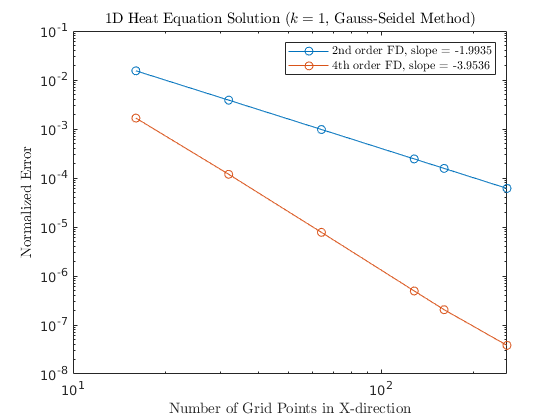
\includegraphics[width=1.0\linewidth]{dim1_GS.png}
        \caption{1D problem}
    \label{fig:conv1d}
    \end{subfigure}%
    \begin{subfigure}[t]{.5\textwidth}
        \centering
        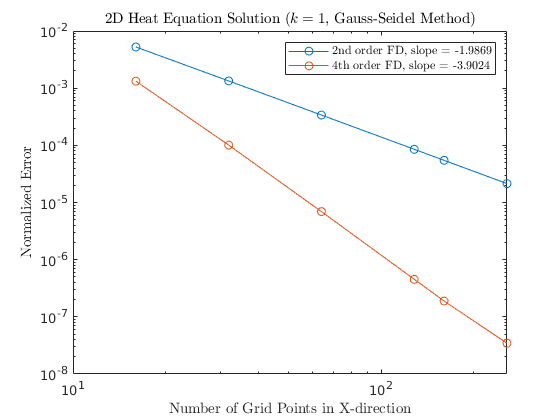
\includegraphics[width=1.0\linewidth]{dim2_GS.png}
        \caption{2D problem}
    \label{fig:conv2d}
    \end{subfigure}
    \caption{Convergence plot for 1D and 2D problem}
\label{fig:conv}
\end{figure}

\subsection{Runtime performance}
GRVY library is utilized to measure runtime performance. In Figure \ref{fig:timing}, we present the result
for 1D problem, where num\_Mesh = 256, and we use second-order finite difference with Gauss-Seidel method
to solve the linear system. From the result we see that the iterative solver (which updates the solution
vector) takes up most of the time (89\% here), and other part of Solve\_System takes a large part (10\%) too.
In each iteration, besides calling functions to update the solution vector, the subroutine Solve\_System
computes the difference between two iterations, and decides whether to exit loop based on the difference.

\begin{figure}[h]
    \centering
    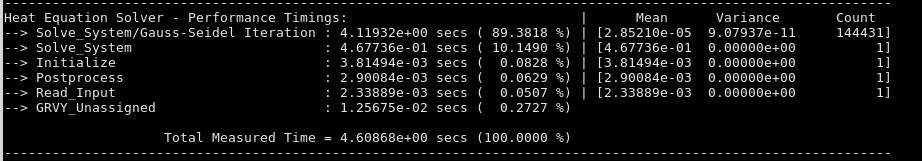
\includegraphics[width=\textwidth]{timing.png}
    \caption{Runtime performance measurements}
    \label{fig:timing}
\end{figure}

\subsection{Code coverage}
We use the gcov/lcov tool for code coverage. A suite of regression tests are run, which includes different
cases: 1D and 2D, second- and fourth-order, Jacobi and Gauss-Seidel method. Figure \ref{fig:code_coverage}
shows our result (before linking to PETSc and HDF5). To reproduce the result, configure with additional flag
``-{}-enable-coverage'', and then run 
\begin{verbatim}
$ make clean
$ make
$ make coverage
\end{verbatim}

In Figure \ref{fig:code_coverage}, note that the source file Sparse\_Matrix\_Mod.f90 has only 65.2\% line
coverage. Further examination reveals that there is a subroutine for outputing sparse matrix that is never
called in our regression tests. This is fine, since the sparse matrix is only printed when we run the
program in verbose output mode (debug\_Flag = 2).

\begin{figure}
    \centering
    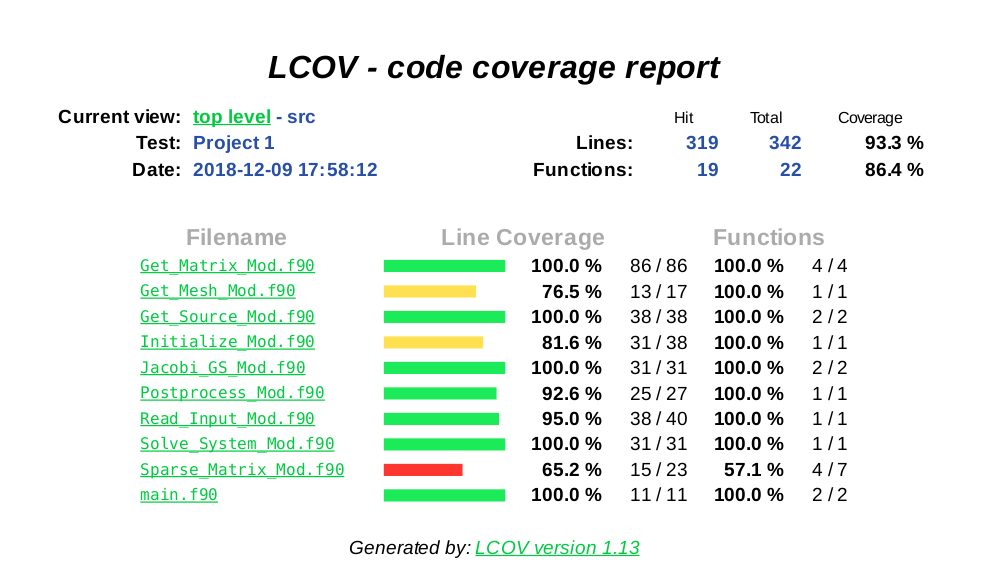
\includegraphics[width=\textwidth]{code_coverage.png}
    \caption{Code coverage report}
    \label{fig:code_coverage}
\end{figure}

\subsection{2D solution plot}
As described in Section 4.3, we use the MASA library to get the source term, and solve for the temperature 
field. Figure \ref{fig:2Dplot}(\subref{fig:2Dplot_numerical}) shows the result for a $32 \times 32$ mesh,
obtained with fourth-order finite difference and Gauss-Seidel method. Figure 
\ref{fig:2Dplot}(\subref{fig:2Dplot_exact}) presents the corresponding analytic temperature field. The
exact temperature field $T(x,y)$ is given by
$$T(x,y) = \cos(2\pi x) \cos(2\pi y)$$
It can be seen that our numerical result is very close to the analytic one.

Tools to produce these 2D plots: We use MATLAB's plotting utilities. First, read the data using function
``h5read''. Then plot with function ``contourf''. The labels and title are set with MATLAB functions as
well.

\begin{figure}[ht]
    \centering
    \begin{subfigure}[t]{.5\textwidth}
        \centering
        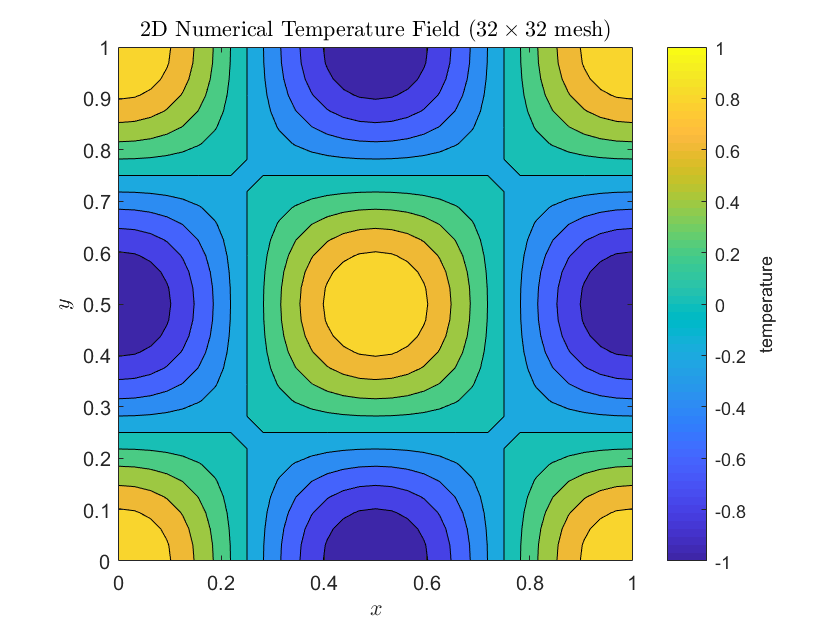
\includegraphics[width=1.0\linewidth]{solution_plot2D.png}
        \caption{Numerical temperature field}
    \label{fig:2Dplot_numerical}
    \end{subfigure}%
    \begin{subfigure}[t]{.5\textwidth}
        \centering
        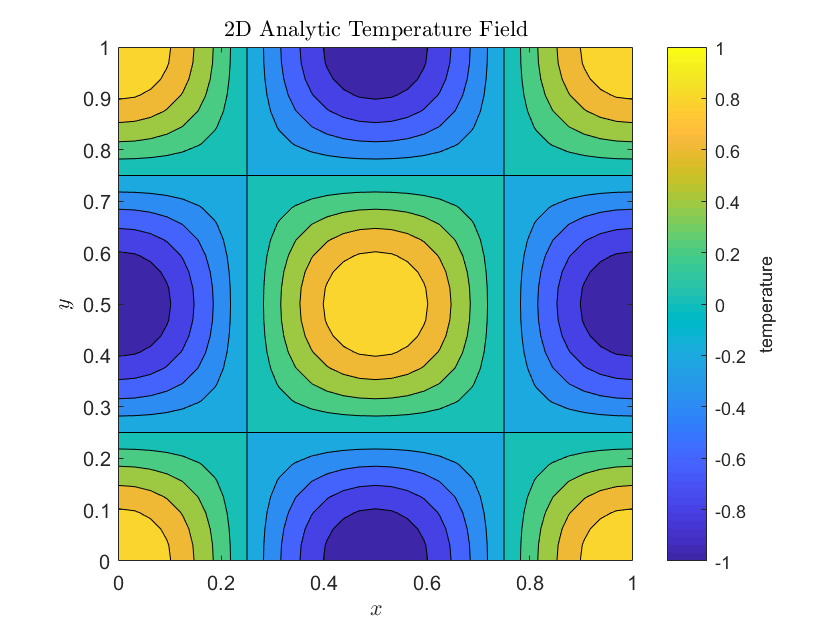
\includegraphics[width=1.0\linewidth]{solution_plot2D_exact.png}
        \caption{Analytic temperature field}
    \label{fig:2Dplot_exact}
    \end{subfigure}
    \caption{2D solution plot}
\label{fig:2Dplot}
\end{figure}


\section{PETSc Implementation}
In addition to the internal Jacobi and Gauss-Seidel solvers, our application include (optional) support
to use PETSc's GMRES solver. To enable PETSc solver, configure with an additional option
``-{}-with-petsc=\$PETSC\_DIR'', and make sure to load module ``gcc'' and ``petsc/3.9-uni''. For convenience,
the configure lines are reproduced below:

\begin{verbatim}
$ module load boost hdf5
$ module load gcc 
$ module load petsc/3.9-uni
$ export PKGPATH=/work/00161/karl/stampede2/public/
$ ./configure FC=mpif90 FCFLAGS=`-g -O0 -Wall' --with-masa=$PKGPATH/masa-gnu7-0.50 \
    --with-grvy=$PKGPATH/grvy-gnu7-0.34 --with-hdf5=$TACC_HDF5_DIR \
    --with-petsc=$PETSC_DIR
\end{verbatim}
Then run ``make'' to build our program. The PETSc solver's tolerances can be set via command line:

\begin{verbatim}
$ ./heateq input.dat -ksp_atol <abtol> -ksp_rtol <rtol> -ksp_max_it <maxits>
\end{verbatim}
where ``abtol'' is the absolute tolerance, ``rtol'' is the relative tolerance, and ``maxits'' is maximum
iterations. The default values are $1\times 10^{-50}$, $1\times 10^{-7}$, 10000, respectively.

\subsection{Verification of PETSc solver}
We redo the uniform mesh refinement study as before, and compare the PETSc result with our internal solvers.
Table \ref{table:petsc_verification} shows the normalized error compared to MASA solution for 1D problem,
second-order scheme. It can be seen that the results from PETSc and Gauss-Seidel are very close (the same in
first four digits). Therefore the solution using PETSc also follows the same $O(h^2)$ convergence rate.
Hence our implementation of PETSc is trustworthy.

\begin{table}[h]
\centering
\begin{tabular}{c|c|c|c|c|c}
    \hline
    num\_Mesh & 16 & 32 & 64 & 128 & 256\\
    \hline
    Gauss-Seidel   & 1.539E-2 & 3.882E-3 & 9.766E-4 & 2.450E-4 & 6.136E-4     \\
    \hline
    PETSc   & 1.539E-2 & 3.882E-3 & 9.766E-4 & 2.450E-4 & 6.136E-5  \\
    \hline
\end{tabular}
\caption{Normalized error compared to MASA for 1D problem, second-order scheme}
\label{table:petsc_verification}
\end{table}


\subsection{Comparison of runtime performance}
We compare the runtime performance of GMRES method from PETSc with Jacobi and Gauss-Seidel methods written
by ourselves. As shown in Figure \ref{fig:performance}, GMRES is slower than Jacobi and Gauss-Seidel method
when the number of grid points is small, which is due to the overhead of preparing PETSc objects; However, it
scales much better to larger-size problems.

\begin{figure}[ht]
    \centering
    \begin{subfigure}[t]{.5\textwidth}
        \centering
        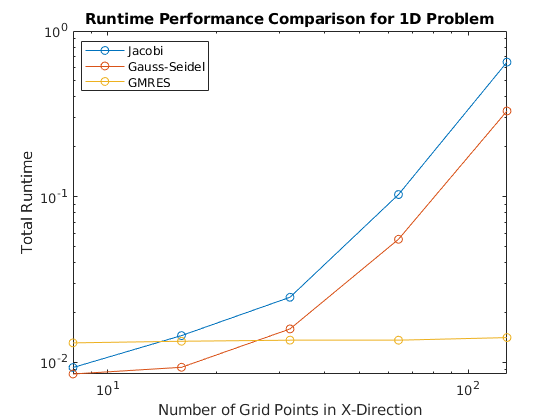
\includegraphics[width=1.0\linewidth]{perfomance_1D.png}
        \caption{1D problem}
    \label{fig:performance_1D}
    \end{subfigure}%
    \begin{subfigure}[t]{.5\textwidth}
        \centering
        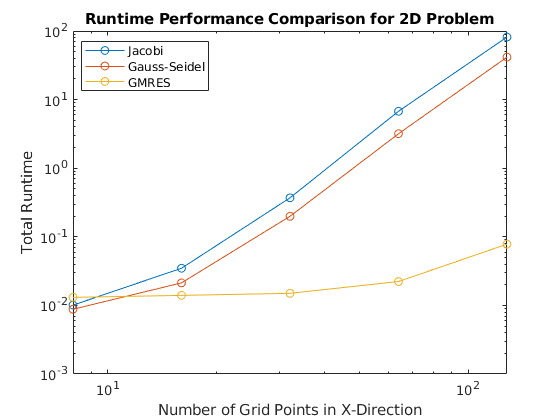
\includegraphics[width=1.0\linewidth]{performance_2D.png}
        \caption{2D problem}
    \label{fig:performance_2D}
    \end{subfigure}
    \caption{Comparison of total runtime for second-order scheme}
\label{fig:performance}
\end{figure}

\end{document}